
%\noindent This document provides a foundation of concepts for using interaction terms in regression.  \\








%_____
\pagebreak
\section*{Interaction terms}

Prerequisites: Sections~1.1-1.6, 3.1, 4.1-4.4, 7.1-7.4, and~8.1 from \href{http://www.openintro.org/stat/textbook.php}{OpenIntro Statistics} are the bare minimum.

\begin{example}{Suppose we were to conduct an experiment where we measured the effect of water and sunlight on plant growth. While each of these contributes individually to plant growth, we might wonder whether there is any interaction between them when promoting growth.}
First and foremost, we would notice no amount of water is sufficient for plant growth if sunshine is completely absent, and vice versa. If you modeled growth simply as a function of sunshine plus water (for example, using a basic multiple regression model introduced in Chapter~8 of \href{http://www.openintro.org/stat/textbook.php}{OpenIntro Statistics}), you'd run into trouble at first. This section tackles this challenge through the use of interaction terms in the context of multiple regression.
\end{example}

Let's consider an experiment that examines the impact of Vitamin C from two sources on the growth of teeth in Guinea pigs.\footnote{Bliss CI. 1952. The Statistics of Bioassay. \emph{Academic Press}. We'll consider a subset of the data available (excludes dose level 0.5), which can be accessed in R via the \data{ToothGrowth} data set.} In this experiment, each Guinea pig was randomly assigned to one of two possible levels of each variable:
\begin{itemize}
\setlength{\itemsep}{0mm}
\item \var{supp} indicates a supplement type for Vitamin C, with levels \resp{VC} for ascorbic acid and \resp{OJ} for orange juice.
\item \var{dose} indicates the amount of Vitamin C, which takes values of either 1~or~2~mg.
\end{itemize}
The researchers measured the length of the teeth of the Guinea pigs as the experimental outcome. The data are summarized in Figure~\ref{interaction}, where each combination of treatments was applied to 10 Guinea pigs.

\begin{figure}[h]
\centering
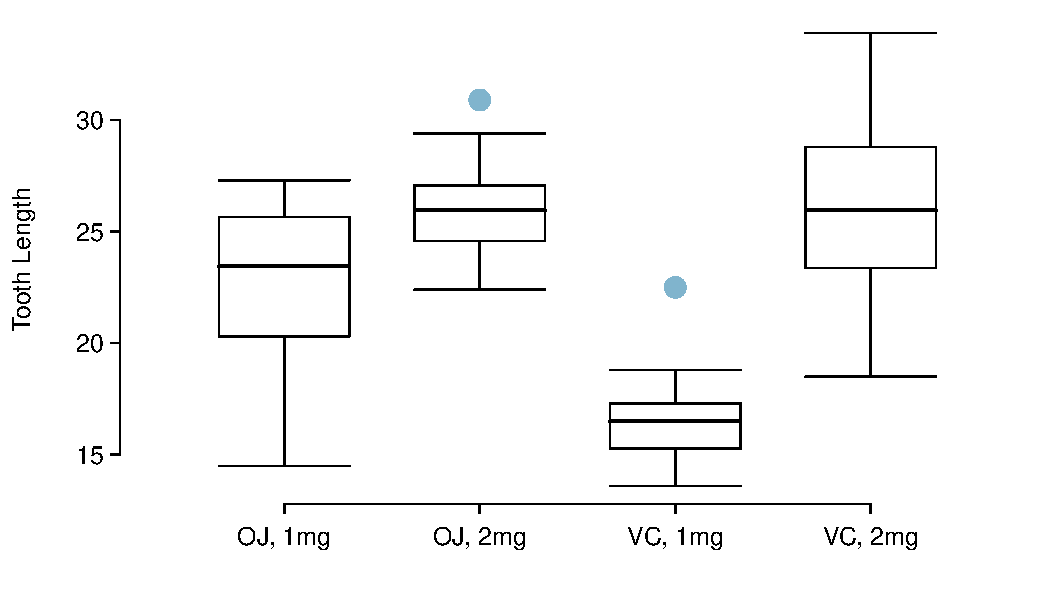
\includegraphics[width=0.9\textwidth]{RegressionExtras/figures/interaction/interaction}
\caption{Side-by-side box plots summarizing the \data{ToothGrowth} data set. Each Guinea pig received a specific amount of Vitamin C (1mg or 2mg) and the source of that Vitamin C was either ascorbic acid (\resp{VC}) or orange juice (\resp{OJ}).}
\label{interaction}
\end{figure}

\begin{tipBox}{\tipBoxTitle{Experiments can randomize along 1 \emph{or more} variables}
In OpenIntro Statistics, we only considered experiments where the researchers randomly assigned one type of treatment. However, by randomizing more treatments, we can identify causal relationships among a set of variables. The example in this section takes a small step into the field of statistics called \term{experimental design}.}
\end{tipBox}



Our aim is to build a multiple regression model that accurately estimates the impact of each variable. We will start by building a model of the following form:
\begin{align*}
y = \beta_0 + \beta_{supp}x_{supp} + \beta_{dose}x_{dose} + residuals
\end{align*}
The fitted model is summarized in Table~\ref{interaction-simpleModelSummary}. Notice the slightly different variable name \var{suppVC} in the table (rather than \var{supp}). This new \var{suppVC} variable was automatically generated by the statistical software since \var{supp} was a categorical variable. The new variable takes value 1 when the supplement is \resp{VC} and 0 when the supplement is \resp{OJ}.
\begin{table}
\centering
\begin{tabular}{rrrrr}
  \hline
 & Estimate & Std. Error & t value & Pr($>$$|$t$|$) \\ 
  \hline
(Intercept) & 14.8325 & 2.0319 & 7.30 & 0.0000 \\ 
  suppVC & -2.9250 & 1.2253 & -2.39 & 0.0222 \\ 
  dose & 6.3650 & 1.2253 & 5.19 & 0.0000 \\ 
   \hline
\end{tabular}
\caption{Summary for the multiple regression model for the Guinea pig experiment.}
\label{interaction-simpleModelSummary}
\end{table}

\begin{exercise}\label{writeOutInteractionModelWOInteraction}
Write the model represented by the output shown in Table~\ref{interaction-simpleModelSummary}. The solution is in the footnote.\footnote{$y = 14.83 - 2.93x_{suppVC} + 6.37x_{dose} + residuals$}
\end{exercise}

\begin{exercise}\label{findInteractionNeeded}
Use the model from Exercise~\ref{writeOutInteractionModelWOInteraction} to predict an outcome for each possible combination of variables. Calculate these means and plot them on Figure~\ref{interaction}. The~plot is provided in the footnote.\footnote{The means are represented by red dotted lines.\\\color{white}WWW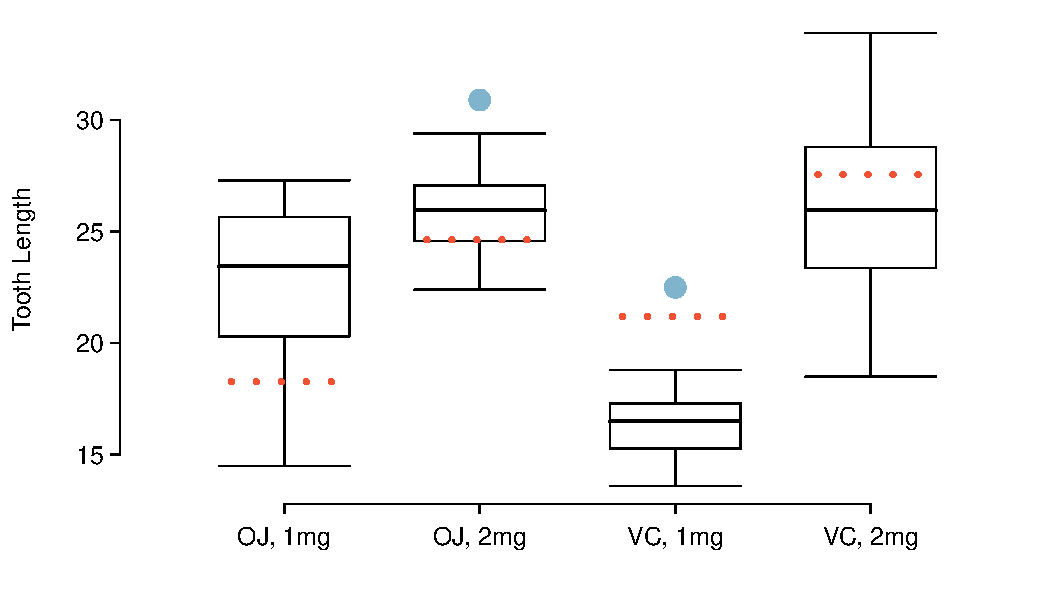
\includegraphics[width=0.7\textwidth]{RegressionExtras/figures/interaction/interaction-noint-w-mean}}
\end{exercise}

Re-examining the solution to Exercise~\ref{findInteractionNeeded}, the fitted values fall far from the centers of the groups, which is a signal that the model does not fit the data very well.

The model you identified in Exercise~\ref{writeOutInteractionModelWOInteraction} assumes that the effects of the supplement and dose are independent. However, it is also possible that the two treatments interact, i.e. the effect of one may partially depend on the value of the other. We can model this \term{interaction} effect using a new term:
\begin{align*}
y = \beta_0 + \beta_{suppVC}x_{suppVC} + \beta_{dose}x_{dose} + \beta_{suppVC:dose}x_{suppVC}x_{dose} + residuals
\end{align*}
The term $\beta_{suppVC:dose}x_{suppVC}x_{dose}$ represents the interaction. The summary for this model is shown in Table~\ref{modelSummaryIncludingInteraction}, and the interaction term is indeed statistically significant.
\begin{table}[ht]
\centering
\begin{tabular}{rrrrr}
  \hline
 & Estimate & Std. Error & t value & Pr($>$$|$t$|$) \\ 
  \hline
(Intercept) & 19.3400 & 2.5419 & 7.61 & 0.0000 \\ 
  suppVC & -11.9400 & 3.5948 & -3.32 & 0.0021 \\ 
  dose & 3.3600 & 1.6076 & 2.09 & 0.0437 \\ 
  suppVC:dose & 6.0100 & 2.2735 & 2.64 & 0.0121 \\ 
   \hline
\end{tabular}
\caption{Summary for the multiple regression model with the interaction term.}
\label{modelSummaryIncludingInteraction}
\end{table}

\begin{exercise} \label{identifyModelWInteraction}
Write the model summarized by Table~\ref{modelSummaryIncludingInteraction}. The solution is in the footnote.\footnote{$y = 19.34  - 11.94x_{suppVC} + 3.36 x_{dose} + 6.01 x_{suppVC}x_{dose} + residuals$ (could also use $x_{suppVC:dose}$ in place of $x_{suppVC}x_{dose}$).}
\end{exercise}

\begin{exercise} \label{CalculatedPredictedMeans}
Using the model equation you generated in Exercise~\ref{identifyModelWInteraction}, calculate the predicted value for a new observation for each group. The solution is in the footnote.\footnote{Consider the predicted value for $y$ under each of the four possible supplement/dose scenarios:
\begin{itemize}
\setlength{\itemsep}{0mm}
\item Orange juice and dosage of 1mg ($x_{suppVC}=0, x_{dose}=1$)
	\begin{align*}
	\hat{y} &= \beta_0 + \beta_{suppVC}x_{suppVC} +
			\beta_{dose}x_{dose} +
			\beta_{suppVC:dose}x_{suppVC}x_{dose} \\
		&= \beta_0 + \beta_{suppVC}\times 0 +
			\beta_{dose}\times 1 +
			\beta_{suppVC:dose}\times 0\times 1 \\
		&= \beta_0 + \beta_{dose}
		\sim b_0 + b_{dose}
		= 22.70
	\end{align*}
\item Orange juice and dosage of 2mg ($x_{suppVC}=0, x_{dose}=2$)
	\begin{align*}
	\hat{y} &= \beta_0 + \beta_{suppVC}x_{suppVC} +
			\beta_{dose}x_{dose} +
			\beta_{suppVC:dose}x_{suppVC}x_{dose} \\
		&= \beta_0 + \beta_{suppVC}\times 0 +
			\beta_{dose}\times 2 +
			\beta_{suppVC:dose}\times 0\times 2 \\
		&= \beta_0 + 2\beta_{dose}
		= b_0 + 2b_{dose}
		= 26.06
	\end{align*}
\item Ascorbic acide and dosage of 1mg ($x_{suppVC}=1, x_{dose}=1$)
	\begin{align*}
	\hat{y} &= \beta_0 + \beta_{suppVC}x_{suppVC} +
			\beta_{dose}x_{dose} +
			\beta_{suppVC:dose}x_{suppVC}x_{dose} \\
		&= \beta_0 + \beta_{suppVC}\times 1 +
			\beta_{dose}\times 1 +
			\beta_{suppVC:dose}\times 1\times 1 \\
		&= \beta_0 + \beta_{suppVC} + \beta_{dose} +
			\beta_{suppVC:dose}
		= b_0 + b_{suppVC} + b_{dose} +
			b_{suppVC:dose}
		= 16.77
	\end{align*}
\item Ascorbic acide and dosage of 2mg ($x_{suppVC}=1, x_{dose}=2$)
	\begin{align*}
	\hat{y} &= \beta_0 + \beta_{suppVC}x_{suppVC} +
			\beta_{dose}x_{dose} +
			\beta_{suppVC:dose}x_{suppVC}x_{dose} \\
		&= \beta_0 + \beta_{suppVC}\times 1 +
			\beta_{dose}\times 2 +
			\beta_{suppVC:dose}\times 1\times 2 \\
		&= \beta_0 + \beta_{suppVC} + 2\beta_{dose} +
			2\beta_{suppVC:dose}
		= b_0 + b_{suppVC} + 2b_{dose} +
			2b_{suppVC:dose}
		= 26.14
	\end{align*}
\end{itemize}}
\end{exercise}

%A sharp eye will notice that the means calculated in Exercise~\ref{CalculatedPredictedMeans} are the same means for each of the four possible treatment combinations. The model with the interaction can fully adjust for differences among the groups, and since the best guess at a future value is the mean, the model calculates the best estimates of the $\beta_i$ terms using the group means.







\pagebreak

\begin{exercise}
Suppose we were to run an experiment where 24 bean plants are randomized into one of four groups:
\begin{itemize}
\setlength{\itemsep}{0mm}
\item Each plant receives 1~teaspoon of water and 1~hour of sunlight each~day.
\item Each plant receives 4~tablespoons of water and 1~hour of sunlight each~day.
\item Each plant receives 1~teaspoon of water and 8~hours of sunlight each~day.
\item Each plant receives 4~tablespoons of water and 8~hours of sunlight each~day.
\end{itemize}
\begin{enumerate}[(a)]
\item Which group do you think will have the least plant growth?
\item The most plant growth?
\item How confident are you in your answers?
\item Do you think the effects of the water and sunlight on plans are independent? If so, explain why. If not, explain how you might model this relationship.
\end{enumerate}
\end{exercise}





%_____
%\pagebreak
%\section{Prediction of the mean response}



%_____
%\pagebreak
%\section{Prediction of future values}

%Note the extreme importance of the normality assumption regarding the residuals.




































